\chapter{Технологический раздел}

В данном разделе выбраны средства разработки программного обеспечения, показаны детали реализации, а также выбраны гиперпараметры модели, с которыми модель работает наилучшим образом с точки зрения выбранного функционала качества.

\section{Средства реализации ПО}
В качестве языка программирования был использован язык Python \cite{bib:python}, поскольку этот язык кроссплатформенный и для него разработано огромное количество библиотек и модулей, решающих разнообразные задачи. 

В частности, имеется библиотека, включающая в себя алгоритм градиентного бустинга, а также вычисление метрики MAPE в библиотеке sklearn \cite{bib:sklearn}.

Для работы с табличными данными была выбрана библиотека pandas \cite{bib:pandas}, так как она имеет мощные функции для обработки данных, интеграцию с другими библиотеками, а также поддержку чтения и записи различных форматов данных.

Для создания графиков были выбраны библиотеки matplotlib \cite{bib:matplotlib} и seaborn \cite{bib:seaborn}, доступные на языке Python, так как они предоставляет удобный интерфейс для работы с данными и их визуализации.


\section{Листинг}
В листинге \ref{lst:gen1} представлен код, решающий задачу регрессии.

\begin{lstlisting}[label=lst:gen1,caption=Код для решения задачи регрессии]
import pandas as pd
import numpy as np
from sklearn.model_selection import train_test_split
from sklearn.preprocessing import LabelEncoder
from sklearn.ensemble import  GradientBoostingRegressor

data = pd.read_csv('students.csv')
le = LabelEncoder()
for col in data.columns:
    data[col] = le.fit_transform(data[col])
X = data.drop(['G3', 'G2', 'G1', 'school'], axis=1)
y = data['G3']
X_train, X_test, y_train, y_test = train_test_split(X, y, test_size=0.2, random_state=42)
model = GradientBoostingRegressor(learning_rate = 0.01, max_depth=9, n_estimators = 500, subsample = 0.5)
model.fit(X_train, y_train)
y_pred = model.predict(X_test)
s = 0
cnt = 0
y_test = y_test.values
y_pred = y_pred
for i in range(len(y_test)):
    if y_test[i] > 0.1:
        s += abs(y_test[i] - y_pred[i]) / y_test[i]
        cnt += 1
print(s / cnt * 100)

\end{lstlisting}

\section{Выбор гиперпараметров модели}

Опишем параметры модели GradientBoostingRegressor из библиотеки sklearn \cite{bib:sklearn}:
\begin{enumerate}
    \item learning\_rate: 
    \begin{itemize}
        \item Определяет вклад каждого дерева в общий результат. Чем ниже learning rate, тем меньше влияние каждого дерева.
        \item Диапазон: [0, +inf].
        \item Более низкий learning rate требует большего количества деревьев для достижения хорошей точности, но может уменьшить переобучение.
    \end{itemize}

    \item n\_estimators:
    \begin{itemize}
        \item Определяет количество деревьев (или итераций), которые будут добавлены к модели.
        \item Диапазон: любое положительное целое число.
        \item Большее количество деревьев может улучшить точность модели, но также увеличивает время обучения.
    \end{itemize}
    \item subsample
    \begin{itemize}
        \item Определяет долю обучающих данных, используемых для построения каждого дерева.
        \item Диапазон: (0, 1].
        \item Уменьшение значения subsample может уменьшить переобучение, но снизит скорость обучения.
    \end{itemize}
    \item max\_depth
    \begin{itemize}
        \item Определяет максимальную глубину каждого дерева.
        \item Диапазон: любое положительное целое число.
        \item Большая глубина деревьев может привести к переобучению, но также может улучшить точность модели.
    \end{itemize}
\end{enumerate}

Параметры модели GradientBoostingRegressor позволяют настраивать модель для достижения оптимального баланса между точностью и предотвращением переобучения.

Проварьируем эти параметры с использованием следующих значений:
\begin{itemize}
    \item learning\_rate: [0.0001, 0.01, 0.1]; 
    \item n\_estimators: [10, 500, 1000];
    \item subsample: [0.05, 0.5, 0.8];
    \item max\_depth: [5, 9, 12].
\end{itemize}

В результате, получаем таблицы \ref{tbl_comp_1}-\ref{tbl_comp_2}.
\newpage

\begin{table}[h!]
	\begin{center}
		\caption{\label{tbl_comp_1}Cравнение ошибки при разных гиперпараметрах (часть 1)} 
		\footnotesize
		\begin{tabular}{|l|l|l|l|l|}
			\hline	
   \multicolumn{1}{|c|}{\begin{tabular}[c]{@{}c@{}}learning\_rate \end{tabular}} & 
    \multicolumn{1}{c|}{\begin{tabular}[c]{@{}c@{}} n\_estimators \end{tabular}} & 
    \multicolumn{1}{c|}{\begin{tabular}[c]{@{}c@{}}subsample \end{tabular}} & 
   \multicolumn{1}{c|}{\begin{tabular}[c]{@{}c@{}}max\_depth\end{tabular}}  & 
    \multicolumn{1}{c|}{\begin{tabular}[c]{@{}c@{}}MAPE\end{tabular}} \\
\hline 0.05 & 10 & 5 & 0.0001 & 24.2 \\
\hline 0.05 & 10 & 5 & 0.0100 & 24.0 \\
\hline 0.05 & 10 & 5 & 0.1000 & 22.7 \\
\hline 0.05 & 10 & 9 & 0.0001 & 24.2 \\
\hline 0.05 & 10 & 9 & 0.0100 & 23.7 \\
\hline 0.05 & 10 & 9 & 0.1000 & 22.8 \\
\hline 0.05 & 10 & 12 & 0.0001 & 24.2 \\
\hline 0.05 & 10 & 12 & 0.0100 & 23.8 \\
\hline 0.05 & 10 & 12 & 0.1000 & 22.9 \\
\hline 0.05 & 500 & 5 & 0.0001 & 23.9 \\
\hline 0.05 & 500 & 5 & 0.0100 & 21.1 \\
\hline 0.05 & 500 & 5 & 0.1000 & 33.9 \\
\hline 0.05 & 500 & 9 & 0.0001 & 23.9 \\
\hline 0.05 & 500 & 9 & 0.0100 & 20.9 \\
\hline 0.05 & 500 & 9 & 0.1000 & 32.9 \\
\hline 0.05 & 500 & 12 & 0.0001 & 23.9 \\
\hline 0.05 & 500 & 12 & 0.0100 & 21.6 \\
\hline 0.05 & 500 & 12 & 0.1000 & 36.3 \\
\hline 0.05 & 1000 & 5 & 0.0001 & 23.7 \\
\hline 0.05 & 1000 & 5 & 0.0100 & 22.1 \\
\hline 0.05 & 1000 & 5 & 0.1000 & 45.6 \\
\hline 0.05 & 1000 & 9 & 0.0001 & 23.6 \\
\hline 0.05 & 1000 & 9 & 0.0100 & 21.9 \\
\hline 0.05 & 1000 & 9 & 0.1000 & 39.4 \\
\hline 0.05 & 1000 & 12 & 0.0001 & 23.6 \\
\hline 0.05 & 1000 & 12 & 0.0100 & 22.8 \\
\hline 0.05 & 1000 & 12 & 0.1000 & 44.7 \\
\hline 0.50 & 10 & 5 & 0.0001 & 24.2 \\
\hline 0.50 & 10 & 5 & 0.0100 & 23.4 \\
\hline 0.50 & 10 & 5 & 0.1000 & 21.0 \\
\hline 0.50 & 10 & 9 & 0.0001 & 24.1 \\
\hline 0.50 & 10 & 9 & 0.0100 & 23.2 \\
\hline 0.50 & 10 & 9 & 0.1000 & 21.2 \\
\hline
	\end{tabular}
	\end{center}
\end{table}

\newpage

\begin{table}[h!]
	\begin{center}
		\caption{\label{tbl_comp_2}Cравнение точности при разных гиперпараметрах (часть 2)} 
		\footnotesize
		\begin{tabular}{|l|l|l|l|l|}
			\hline	
   \multicolumn{1}{|c|}{\begin{tabular}[c]{@{}c@{}}learning\_rate \end{tabular}} & 
    \multicolumn{1}{c|}{\begin{tabular}[c]{@{}c@{}} n\_estimators \end{tabular}} & 
    \multicolumn{1}{c|}{\begin{tabular}[c]{@{}c@{}}subsample \end{tabular}} & 
   \multicolumn{1}{c|}{\begin{tabular}[c]{@{}c@{}}max\_depth\end{tabular}}  & 
    \multicolumn{1}{c|}{\begin{tabular}[c]{@{}c@{}}MAPE\end{tabular}} \\
\hline 0.50 & 10 & 12 & 0.0001 & 24.1 \\
\hline 0.50 & 10 & 12 & 0.0100 & 23.3 \\
\hline 0.50 & 10 & 12 & 0.1000 & 22.3 \\
\hline 0.50 & 500 & 5 & 0.0001 & 23.7 \\
\hline 0.50 & 500 & 5 & 0.0100 & 21.2 \\
\hline 0.50 & 500 & 5 & 0.1000 & 24.4 \\
\hline 0.50 & 500 & 9 & 0.0001 & 23.7 \\
\hline 0.50 & 500 & 9 & 0.0100 & 20.9 \\
\hline 0.50 & 500 & 9 & 0.1000 & 21.4 \\
\hline 0.50 & 500 & 12 & 0.0001 & 23.7 \\
\hline 0.50 & 500 & 12 & 0.0100 & 21.0 \\
\hline 0.50 & 500 & 12 & 0.1000 & 23.2 \\
\hline 0.50 & 1000 & 5 & 0.0001 & 23.4 \\
\hline 0.50 & 1000 & 5 & 0.0100 & 22.0 \\
\hline 0.50 & 1000 & 5 & 0.1000 & 22.6 \\
\hline 0.50 & 1000 & 9 & 0.0001 & 23.3 \\
\hline 0.50 & 1000 & 9 & 0.0100 & 21.2 \\
\hline 0.50 & 1000 & 9 & 0.1000 & 22.9 \\
\hline 0.50 & 1000 & 12 & 0.0001 & 23.3 \\
\hline 0.50 & 1000 & 12 & 0.0100 & 21.2 \\
\hline 0.50 & 1000 & 12 & 0.1000 & 23.2 \\
\hline 0.80 & 10 & 5 & 0.0001 & 24.2 \\
\hline 0.80 & 10 & 5 & 0.0100 & 23.3 \\
\hline 0.80 & 10 & 5 & 0.1000 & 20.9 \\
\hline 0.80 & 10 & 9 & 0.0001 & 24.2 \\
\hline 0.80 & 10 & 9 & 0.0100 & 23.3 \\
\hline 0.80 & 10 & 9 & 0.1000 & 21.5 \\
\hline 0.80 & 10 & 12 & 0.0001 & 24.2 \\
\hline 0.80 & 10 & 12 & 0.0100 & 23.4 \\
\hline 0.80 & 10 & 12 & 0.1000 & 21.7 \\
\hline 0.80 & 500 & 5 & 0.0001 & 23.7 \\
\hline 0.80 & 500 & 5 & 0.0100 & 20.8 \\
\hline 0.80 & 500 & 5 & 0.1000 & 22.5 \\
\hline 0.80 & 500 & 9 & 0.0001 & 23.7 \\
\hline 0.80 & 500 & 9 & 0.0100 & 20.8 \\
\hline 0.80 & 500 & 9 & 0.1000 & 21.7 \\
\hline 0.80 & 500 & 12 & 0.0001 & 23.7 \\
\hline 0.80 & 500 & 12 & 0.0100 & 21.2 \\
\hline 0.80 & 500 & 12 & 0.1000 & 22.5 \\
\hline 0.80 & 1000 & 5 & 0.0001 & 23.4 \\
\hline 0.80 & 1000 & 5 & 0.0100 & 21.7 \\
\hline 0.80 & 1000 & 5 & 0.1000 & 22.6 \\
\hline 0.80 & 1000 & 9 & 0.0001 & 23.4 \\
\hline 0.80 & 1000 & 9 & 0.0100 & 21.2 \\
\hline 0.80 & 1000 & 9 & 0.1000 & 21.4 \\
\hline 0.80 & 1000 & 12 & 0.0001 & 23.4 \\
\hline 0.80 & 1000 & 12 & 0.0100 & 21.2 \\
\hline 0.80 & 1000 & 12 & 0.1000 & 22.4 \\
\hline
	\end{tabular}
	\end{center}
\end{table}

Видим, что наименьшая ошибка модели с точки зрения выбранного функционала качества достигается при следующих параметрах модели:

\begin{itemize}
    \item learning\_rate: 0.01;
    \item n\_estimators: 500;
    \item subsample: 0.80;
    \item max\_depth: 9.
\end{itemize}

На рисунке \ref{fig:imp} построена гистограмма важности признаков построенной модели (важность определяется как нормализованное общее снижение энтропии с помощью этого признака -- индекс Джини). Видно, что наиболее важными признаками для опредлеления выпускного балла являются количество неудач на контрольных и количество прогулов, что логично.

\begin{figure}[h!]
	\centering
	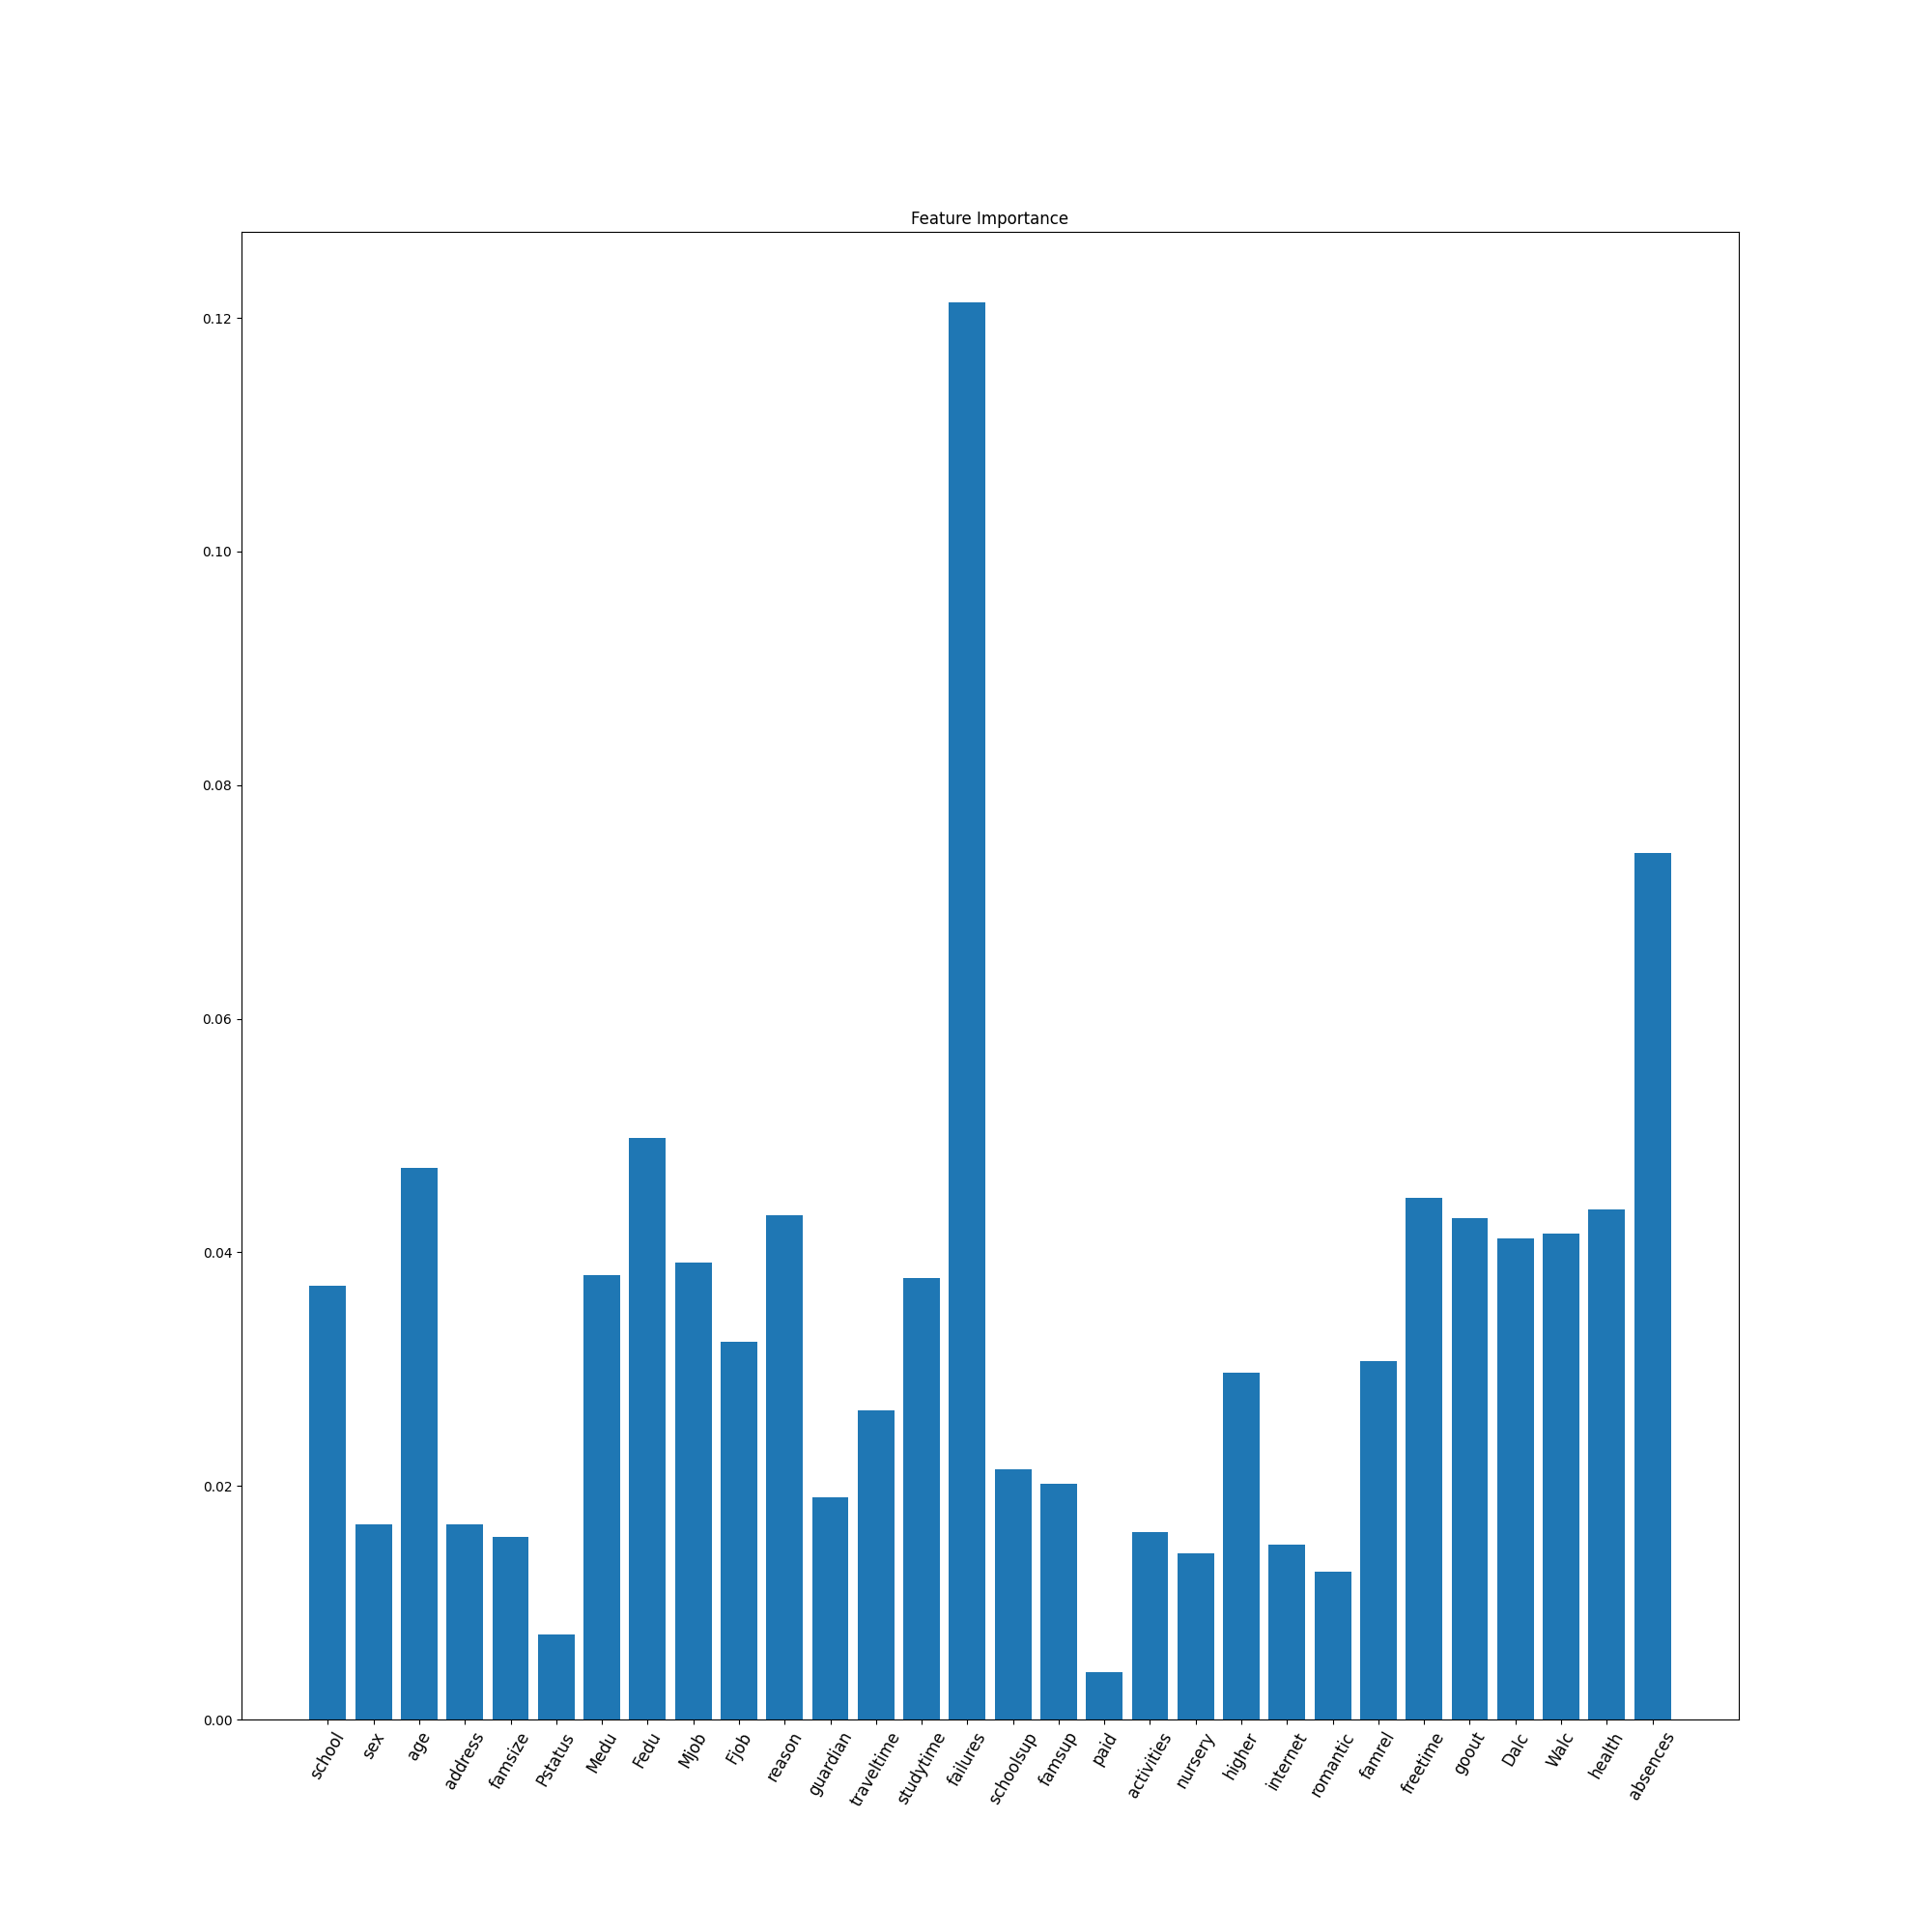
\includegraphics[scale = 0.3]{img/importancies_GradientBoostingRegressor.png}
	\caption{Важность признаков}
	\label{fig:imp}
\end{figure}

Итоговая ошибка модели на тестовой выборке составляет 20.8\%. 

\section{Обобщающая способность}
Оценим обобщающую способность модели. Для этого будем менять каждый из гиперпараметров так, что остальные остаются равными выбранным с помощью функционала качества на тестовой выборке в предыдщем пункте. 


\begin{figure}[h!]
	\centering
	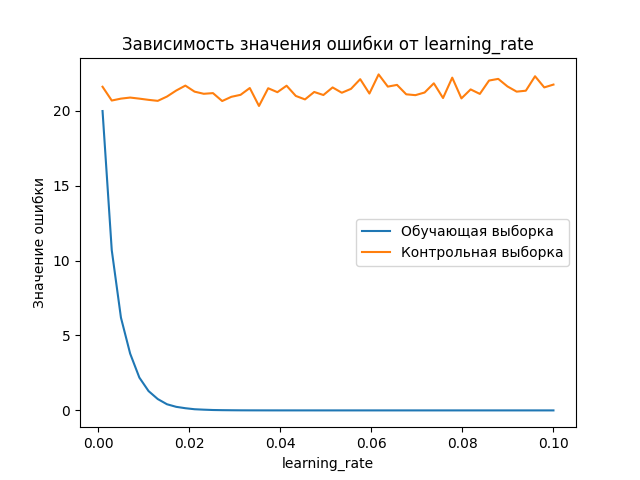
\includegraphics[scale = 0.8]{img/research_learning_rate.png}
	\caption{Зависимость ошибки от learning\_rate}
	\label{fig:lr}
\end{figure}

\begin{figure}[h!]
	\centering
	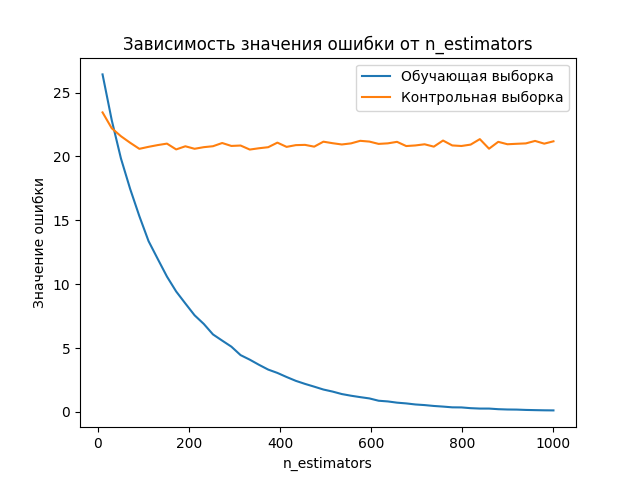
\includegraphics[scale = 0.8]{img/research_n_estimators.png}
	\caption{Зависимость ошибки от n\_estimators}
	\label{fig:ne}
\end{figure}

\begin{figure}[h!]
	\centering
	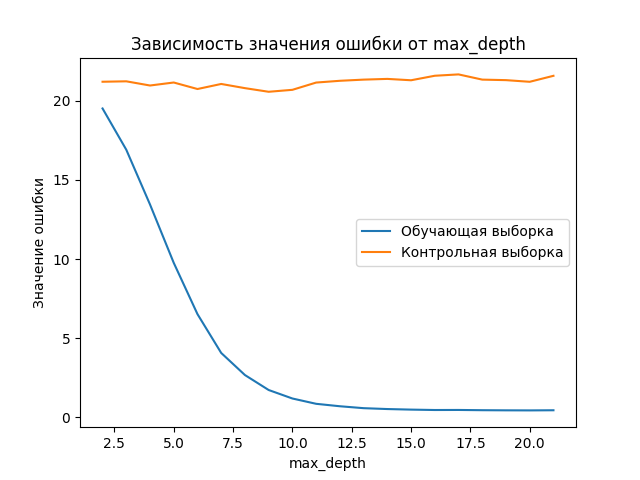
\includegraphics[scale = 0.8]{img/research_max_depth.png}
	\caption{Зависимость ошибки от max\_depth}
	\label{fig:md}
\end{figure}
\newpage
\begin{figure}[h!]
	\centering
	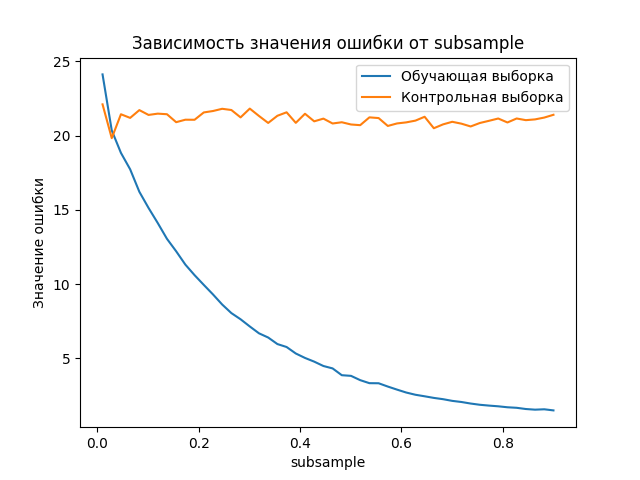
\includegraphics[scale = 0.8]{img/research_subsample.png}
	\caption{Зависимость ошибки от subsample}
	\label{fig:subsample}
\end{figure}

Видим, что обобщающую способность модели при выбранных парметрах можно считать удовлетворительной, поскольку при минимуме ошибки на обучающей выборке достигается минимум ошибки на тестовой (считаем, что при увеличении ошибки на тестовой выборке при минимуме на обучающей модель начинает переобучаться).
\section*{Вывод}
\addcontentsline{toc}{section}{Вывод}

В данном разделе были выбраны средства разработки программного обеспечения, показаны детали реализации, а также выбраны гиперпараметры модели, решающей задачу регрессии.